%%=============================================================================
%% Methodologie
%%=============================================================================

\chapter{\IfLanguageName{dutch}{Praktijk onderzoek}{Practical Research}}
\label{ch:Praktijk onderzoek}

%% TODO: Hoe ben je te werk gegaan? Verdeel je onderzoek in grote fasen, en
%% licht in elke fase toe welke stappen je gevolgd hebt. Verantwoord waarom je
%% op deze manier te werk gegaan bent. Je moet kunnen aantonen dat je de best
%% mogelijke manier toegepast hebt om een antwoord te vinden op de
%% onderzoeksvraag.

In hoofdstuk 2 is het onderzoek gestart met een literatuurstudie waarin besproken werd wat REST, JSON, gRPC en Protobufs exact zijn en hoe de interne architectuur van Fashion Society er uitziet.

In dit hoofdstuk gaat het onderzoek verder met een requirementanalyse en een plan van aanpak waarin beschreven wordt hoe de proof-of-concept tot stand komt en wat de resultaten hiervan zijn.

\section{Requirementanalyse}
\label{sec:Requirementanalyse}

In deze analyse worden de functionele en niet-functionele vereisten opgelijst waaraan een alternatieve implementatie van de Discovery API moet voldoen.

Functionele requirements:
\begin{itemize}
    \item Implementatie aan de hand van .NET Core 3.1 voor long-term support.
    \item Moet een grote hoeveelheid aan parallelle requests kunnen afhandelen.

\end{itemize}

Niet-functionele requirements:
\begin{itemize}
    \item Moet (relatief) gemakkelijk uitbreidbaar zijn.
 \item Moet snel requests kunnen afhandelen.
     \item Moet schaalbaar zijn.
\end{itemize}



\section{Plan van aanpak}
\label{sec:Plan van aanpak}

\subsection{Opstellen van gRPC service in .NET Core 3.1 }
\label{subsec:Opstellen van gRPC service in .NET Core 3.1}
Uit de requirementanalyse kan afgeleid worden dat de service zal moeten draaien in .NET Core 3.1 en niet in .NET Core 5.0 omdat deze geen long-term support heeft van Microsoft.

Zodanig dat gebruik gemaakt kan worden van de voordelen van gRPC zoals codegeneratie zal het project opgebouwd worden vanuit een grpc service project vanuit Visual Studio zelf, dit project bevat de Grpc.AspNetCore package die alles gRPC gerelateerd afhandelt.

Voor de logica in de twee endpoints GetService en GetServiceUrl die respectievelijk een service object en een service url ophalen zal code gerecupereerd worden van de reeds bestaande Discovery API.

De reeds bestaande Discovery API maakt gebruik van het repository patroon voor het ophalen en verwerken van data uit een SQL database in de gRPC service zal dit patroon wegvallen en zal de databasecontext rechtstreeks in de Service geïnjecteerd worden. Uit een verdere analyse van de bestaande code kan er ook geconcludeerd worden dat beide methoden gebruik maken van éénzelfde Get methode in de repository, deze wordt een private methode in de Service die zal worden aangesproken door beide endpoints.

Het protobestand “services.proto” waaruit de bijhorende modellen worden gegenereerd bevat de 2 rpc methodes GetService en GetServiceUrl, beiden hebben deze een input parameter van het messagetype “ServiceName” met als veld een string “name”.
De GetService methode zal een message van het type “ServiceObject” teruggeven, deze bevat de “name”, “address”, “port”, “addNameToUrl” en “hasSwaggerDoc” velden. Deze velden zijn licht afwijkend van het reeds bestaande Model in de Discovery API maar is in samenspraak met mijn co-promotor.
Tot slot is er de GetServiceUrl methode, deze geeft een message van het type “ServiceUrl” terug dewelke een enkel veld bevat zijnde “url”.

In figuur \ref{fig:ProtoPoC} is het gebruikte protobestand te zien.

\begin{figure}[H]
    \centering
    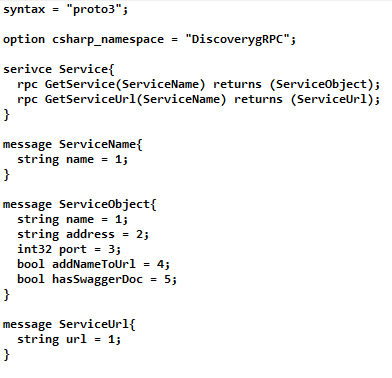
\includegraphics[scale=0.75]{ProtoPoC}
    \caption[Proof-Of-Concept protobestand]{Het gebruikte protobestand}
    \label{fig:ProtoPoC}
\end{figure}

\subsection{Client applicaties voor REST en gRPC}
\label{subsec:Client applicaties voor REST en gRPC}

Om de snelheid van beide implementaties te testen moeten de services worden aangesproken van een client. Hiervoor worden twee identieke implementaties gebruikt in twee Console applicaties (.NET Core). De enige verschillen tussen de twee applicaties zijn de aangesproken endpoints. Deze applicaties zullen aan de hand van een lijst van vier servicenamen calls doen naar de service. Er is voor vier servicenamen gekozen zodanig dat er rekening wordt gehouden met eventuele verschillen in het ophalen van de verschillende data.

Tijdens het gehele proces zal een timer lopen die de totale tijd van de calls zal opnemen.

\subsection{Het verloop van het onderzoek}
\label{subsec:Het verloop van het onderzoek}

Het onderzoek wordt uitgevoerd in drie categorieën, een kleine en grote payload voor het resultaat van parallele requests en een request loop van tienduizend requests voor de response time voor één request te berekenen. In de kleine payload zullen er in totaal vierduizend calls gemaakt worden, elke servicenaam zal tien keer parallel gebruikt worden om vervolgens honderd requests te versturen. In de grote payload zullen er tienduizend calls gemaakt worden en hier zal elke servicenaam vijfentwintig keer parallel gebruikt worden om vervolgens honderd requests te versturen.

Om tot een concreet resultaat van één request te bekomen zal ook deze tienduizend keer worden uitgevoerd. Dit hoge aantal is gekozen om de invloed van eventuele netwerk vertragingen te beperken.
De kleine en grote payload zullen daarintegen vier keer uitgevoerd worden om tot een concreet resultaat te bekomen. Hier zullen eventuele netwerk vertragingen om individuele calls minder doorwegen door het reeds hoge aantal calls in elke uitvoering.


Het CPU gebruik zal manueel in de gaten gehouden worden maar zal in samenspraak met de co-promotor niet in acht genomen worden in de resultaten omdat er geen accurate manier beschikbaar is om het CPU gebruik op de server te registreren.

\section{Resultaat Proof-Of-Concept}
\label{sec:Resultaat Proof-Of-Concept}

\subsection{Single Call}
\label{subsec:Single Call}
Uit het onderzoek is gebleken dat gRPC met ProtocolBuffers voor zowel de GetService methode (-24,06\%) als de GetServiceUrl methode (-23,78\%) sneller is dan REST met JSON.
\begin{figure}[H]
    \centering
    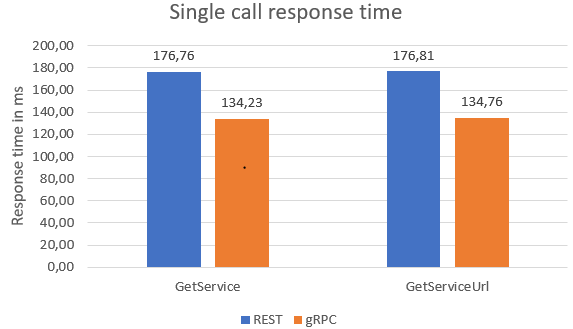
\includegraphics[scale=1]{singleCall}
    \caption[Single Call Response Time]{Resultaat van het onderzoek naar Single call response time.}
    \label{fig:SingleCallResult}
\end{figure}

De verwachting van dit onderdeel was dat het resultaat bij de single call response time een marginaal verschil ging zijn in voordeel van gRPC doordat de response op de calls een kleine hoeveelheid data is voor beide methodes, echter toonde het resultaat een groter dan verwacht verschil in snelheid in voordeel van gRPC.

\subsection{Vierduizend Parallelle Calls}
\label{subsec:Vierduizend parallelle calls}
Uit het onderzoek is gebleken dat gRPC voor zowel de GetService methode (-15,63\%) als voor de GetServiceUrl methode (-20,34\%) sneller is dan REST bij het afhandelen van vierduizend parallelle calls.
\begin{figure}[H]
    \centering
    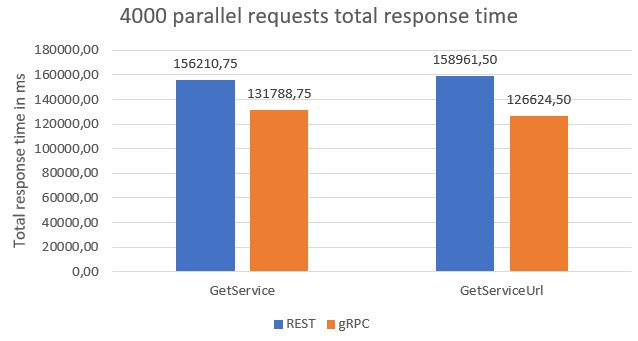
\includegraphics[scale=1]{VierduizendCalls}
    \caption[Resultaten van vierduizend parallelle calls]{Resultaat van het onderzoek naar een kleine hoeveelheid parallelle calls.}
    \label{fig:VierduizendCallsResult}
\end{figure}

Bij dit onderdeel is het resultaat onder de verwachtingen, de verwachtingen waren dat gRPC opmerkelijk sneller ging zijn dan REST door de hoeveelheid aan af te handelen requests. Echter is het gebleken dat dit een verkeerde redenering was voor de verwachting, de hoeveelheid data in de response op elke call blijft namelijk nog altijd klein.

\subsection{Tienduizend Parallelle Calls}
\label{subsec:Tienduizend parallelle calls}
Uit het onderzoek is gebleken dat gRPC voor zowel de GetService methode (-13,96\%) als voor de GetServiceUrl methode (-16,35\%) sneller is dan REST bij het afhandelen van tienduizend parallelle calls.
\begin{figure}[H]
    \centering
    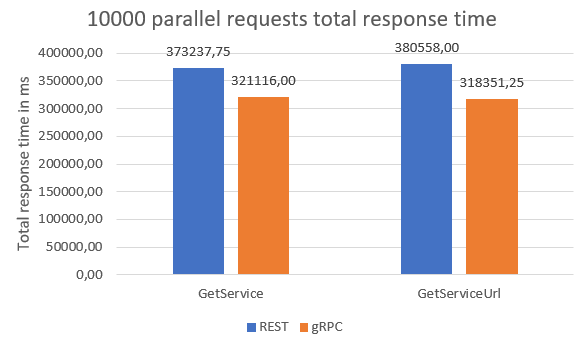
\includegraphics[scale=1]{TienduizendCalls}
    \caption[Resultaten van tienduizend parallelle calls]{Resultaat van het onderzoek naar een grote hoeveelheid parallelle calls.}
    \label{fig:TienduizendCallsResult}
\end{figure}

Net zoals bij de kleine hoeveelheid parallelle calls is het resultaat hier onder de verwachtingen. gRPC is voor zowel de GetService methode (-13,96\%) als voor de GetServiceUrl methode (-16,35\%) sneller dan REST maar ook hier is voor de verwachting dezelfde verkeerde redenering gebruikt als bij de kleine hoeveelheid parallelle calls. Het aantal parallelle calls is wel verhoogd maar de hoeveelheid data in de response op de calls blijft nog altijd hetzelfde.

